\documentclass[12pt]{article}

\usepackage{amsmath, mathtools}
\usepackage{amsfonts}
\usepackage{amssymb}
\usepackage{graphicx}
\usepackage{colortbl}
\usepackage{xr}
\usepackage{hyperref}
\usepackage{longtable}
\usepackage{xfrac}
\usepackage{tabularx}
\usepackage{float}
\usepackage{siunitx}
\usepackage{booktabs}
\usepackage{caption}
\usepackage{pdflscape}
\usepackage{afterpage}


\usepackage[round]{natbib}

%\usepackage{refcheck}

\hypersetup{
    bookmarks=true,         % show bookmarks bar?
      colorlinks=true,       % false: boxed links; true: colored links
    linkcolor=red,          % color of internal links (change box color with linkbordercolor)
    citecolor=green,        % color of links to bibliography
    filecolor=magenta,      % color of file links
    urlcolor=cyan           % color of external links
}

%% Comments

\usepackage{color}

\newif\ifcomments\commentstrue %displays comments
%\newif\ifcomments\commentsfalse %so that comments do not display

\ifcomments
\newcommand{\authornote}[3]{\textcolor{#1}{[#3 ---#2]}}
\newcommand{\todo}[1]{\textcolor{red}{[TODO: #1]}}
\else
\newcommand{\authornote}[3]{}
\newcommand{\todo}[1]{}
\fi

\newcommand{\wss}[1]{\authornote{blue}{SS}{#1}} 
\newcommand{\plt}[1]{\authornote{magenta}{TPLT}{#1}} %For explanation of the template
\newcommand{\an}[1]{\authornote{cyan}{Author}{#1}}

%% Common Parts

\newcommand{\progname}{2D Localizer} % PUT YOUR PROGRAM NAME HERE
\newcommand{\authname}{Aliyah Jimoh} % AUTHOR NAMES                  

\usepackage{hyperref}
    \hypersetup{colorlinks=true, linkcolor=blue, citecolor=blue, filecolor=blue,
                urlcolor=blue, unicode=false}
    \urlstyle{same}
                                


% For easy change of table widths
\newcommand{\colZwidth}{1.0\textwidth}
\newcommand{\colAwidth}{0.15\textwidth}
\newcommand{\colBwidth}{0.82\textwidth}
\newcommand{\colCwidth}{0.1\textwidth}
\newcommand{\colDwidth}{0.05\textwidth}
\newcommand{\colEwidth}{0.8\textwidth}
\newcommand{\colFwidth}{0.17\textwidth}
\newcommand{\colGwidth}{0.5\textwidth}
\newcommand{\colHwidth}{0.28\textwidth}

% Used so that cross-references have a meaningful prefix
\newcounter{defnum} %Definition Number
\newcommand{\dthedefnum}{GD\thedefnum}
\newcommand{\dref}[1]{GD\ref{#1}}
\newcounter{datadefnum} %Datadefinition Number
\newcommand{\ddthedatadefnum}{DD\thedatadefnum}
\newcommand{\ddref}[1]{DD\ref{#1}}
\newcounter{theorynum} %Theory Number
\newcommand{\tthetheorynum}{TM\thetheorynum}
\newcommand{\tref}[1]{TM\ref{#1}}
\newcounter{tablenum} %Table Number
\newcommand{\tbthetablenum}{TB\thetablenum}
\newcommand{\tbref}[1]{TB\ref{#1}}
\newcounter{assumpnum} %Assumption Number
\newcommand{\atheassumpnum}{A\theassumpnum}
\newcommand{\aref}[1]{A\ref{#1}}
\newcounter{goalnum} %Goal Number
\newcommand{\gthegoalnum}{GS\thegoalnum}
\newcommand{\gsref}[1]{GS\ref{#1}}
\newcounter{instnum} %Instance Number
\newcommand{\itheinstnum}{IM\theinstnum}
\newcommand{\iref}[1]{IM\ref{#1}}
\newcounter{reqnum} %Requirement Number
\newcommand{\rthereqnum}{R\thereqnum}
\newcommand{\rref}[1]{R\ref{#1}}
\newcounter{nfrnum} %NFR Number
\newcommand{\rthenfrnum}{NFR\thenfrnum}
\newcommand{\nfrref}[1]{NFR\ref{#1}}
\newcounter{lcnum} %Likely change number
\newcommand{\lthelcnum}{LC\thelcnum}
\newcommand{\lcref}[1]{LC\ref{#1}}
\newcounter{ucnum} %Unlikely change number
\newcommand{\ltheucnum}{LC\theucnum}
\newcommand{\ucref}[1]{UC\ref{#1}}

\usepackage{fullpage}

\newcommand{\deftheory}[9][Not Applicable]
{
\newpage
\noindent \rule{\textwidth}{0.5mm}

\paragraph{RefName: } \textbf{#2} \phantomsection 
\label{#2}

\paragraph{Label:} #3

\noindent \rule{\textwidth}{0.5mm}

\paragraph{Equation:}

#4

\paragraph{Description:}

#5

\paragraph{Notes:}

#6

\paragraph{Source:}

#7

\paragraph{Ref.\ By:}

#8

\paragraph{Preconditions for \hyperref[#2]{#2}:}
\label{#2_precond}

#9

\paragraph{Derivation for \hyperref[#2]{#2}:}
\label{#2_deriv}

#1

\noindent \rule{\textwidth}{0.5mm}

}

\begin{document}

\title{Software Requirements Specification for 2D Localizer} 
\author{Aliyah Jimoh}
\date{\today}
	
\maketitle

~\newpage

\pagenumbering{roman}

\tableofcontents

~\newpage

\section*{Revision History}

\begin{tabularx}{\textwidth}{p{3cm}p{2cm}X}
\toprule {\bf Date} & {\bf Version} & {\bf Notes}\\
\midrule
2025/02/05 & 1.0 & Initial Draft\\
% Date 2 & 1.1 & Notes\\
\bottomrule
\end{tabularx}

~\\

~\newpage

\section{Reference Material}

This section records information for easy reference.

\subsection{Table of Units}

Throughout this document SI (Syst\`{e}me International d'Unit\'{e}s) is employed
as the unit system.  In addition to the basic units, several derived units are
used as described below.  For each unit, the symbol is given followed by a
description of the unit and the SI name.
~\newline

\renewcommand{\arraystretch}{1.2}
% \begin{table}[ht]\caption{Table of Units}
\begin{longtable*}{l l l}
    \toprule		
    \textbf{Symbol} & \textbf{Unit} & \textbf{SI}\\
    \midrule 
    \si{\metre} & length & metre\\\
    \si{\radian} & angle & radians\\
    \bottomrule
  \end{longtable*}
% \end{table}

\subsection{Table of Symbols}

The table that follows summarizes the symbols used in this document along with
their units. The symbols are listed in alphabetical order. 

\renewcommand{\arraystretch}{1.2}
%\noindent \begin{tabularx}{1.0\textwidth}{l l X}
\noindent \begin{longtable*}{l l p{12cm}} \toprule
\textbf{Symbol} & \textbf{Unit} & \textbf{Description}\\
\midrule 
$\mathbf{a_j}$ & \si[per-mode=symbol] {\metre} & Position for beacon $j$
\\
$\mathbf{\tilde{d}}$ & \si[per-mode=symbol] {\metre} & Set of range measurements
\\ 
$\tilde{d_j}$ & \si[per-mode=symbol] {\metre} & Measured range with noise from beacon $j$
\\
$g_j(\mathbf{x_i})$ & \si[per-mode=symbol] {\metre} & Noisy range measurement of robot's position $i$ taken from beacon $j$
\\
$\boldsymbol{\mathcal{I}}$ & \si[per-mode=symbol] {\per\square\metre} & Total Fisher Information Matrix
\\ 
$i$ & \si[per-mode=symbol] {-} & Index for robot's positions
\\
$j$ & \si[per-mode=symbol] {-} & Index for number of beacons
\\ 
$N$ & \si[per-mode=symbol] {-} & Total number of beacons used
\\
$\mathbf{T_{robot}}$ & \si[per-mode=symbol] {\metre} & Pose of robot
\\ 
$\mathbf{x_i}$ & \si[per-mode=symbol] {\metre} & Position $i$th 
\\ 
$\mathbf{\hat{x}}$ & \si[per-mode=symbol] {\metre} & Estimated position for robot
\\ 
$\eta_j$ & \si[per-mode=symbol] {\metre} & Sensor noise 
\\
$\theta$ & \si[per-mode=symbol] {\radian} & Robot's orientation
\\
$\sigma^2_j$ & \si[per-mode=symbol] {\metre} & Noise variance for $j$
\\
\bottomrule
\end{longtable*}

~\newline

\subsection{Abbreviations and Acronyms}

\renewcommand{\arraystretch}{1.2}
\begin{longtable*}{l  l} 
  \toprule		
  \textbf{Abbreviation/Acronym} & \textbf{Definition}\\
  \midrule 
  2D & Two-Dimensional \\
  2D Localizer & 2D Localization Solution\\
  A & Assumption\\
  CRLB & Cram\'er-Rao Lower Bound\\
  DD & Data Definition\\
  FIM & Fisher Information Matrix \\
  FM & Fiducial Marker \\
  GD & General Definition\\
  GS & Goal Statement\\
  IM & Instance Model\\
  LC & Likely Change\\
  MLE & Maximum Likelihood Estimation\\
  PDF & Probability Density Function\\
  PS & Physical System Description\\
  R & Requirement\\
  SE(2) & Special Euclidean Group in 2D \\
  SRS & Software Requirements Specification\\
  TM & Theoretical Model\\
  UC & Unlikely Change\\
  \bottomrule
\end{longtable*}

\subsection{Mathematical Notation}
Throughout this document, there will be typographic conventions as 
well as mathematical operators that are used to distinguish different variables and operations.
~\newline

\renewcommand{\arraystretch}{1.2}
\begin{longtable*}{l  l  l} 
  \toprule		
  \textbf{Notation} & \textbf{Definition} & \textbf{Description}\\
  \midrule 
  $\textbf{A}$ & Matrix & Bold capital letter  \\
  $\textbf{a}$ & Vector & Bold lowercase letter  \\
  $a / A$ & Scalar & Italicized uppercase/lowercase symbol \\
$\lVert~\rVert$ & Euclidean (2) Norm~~~~& Vertical brackets \\
  \bottomrule
\end{longtable*}

\newpage

\pagenumbering{arabic}

\section{Introduction}

Mobile robots have been used to traverse areas with various hazards, help collect data whether through its sensors or obtaining samples, and to overall complete challenging tasks. Due to their autonomy, there is no need to constantly monitor them as they have their own means with interacting with the environment. However, it could raise some concern when there is no reliable method to track their movements, especially if they are placed in a vastly large area or if they are difficult to access once they are operational. Risks such as having difficulty retrieving them if there is a malfunction keeping them from returning or possible collisions in the area or with other robots are reasons one would want to find a way to locate them as they carry out their tasks. The program being documented, 2D Localizer, proposes to solve this problem by developing a 2D localization solution that can implement various sensors to accurately localize the robots as they traverse the map provided.

The following section provides an overview of the Software Requirement Specification (SRS) for 2D Localizer. This section explains the purpose of this document, the scope of the requirements, the characteristics of the intended reader, and the organization of the document.

\subsection{Purpose of Document}

The main purpose of this document is to describe the requirements needed to run 2D Localizer. Information such as the constraints, assumptions and theoretical models used will be provided to help readers get a better understanding of the purpose and computations of this software. Therefore, it can be used as a reference guide on how to plan and set up the requirements needed by the user to get the desired and accurate results.

\subsection{Scope of Requirements} 

The scope of the requirements includes the robot analyzed being in a controlled environment (seen as a 2D environment) to help with potential lighting problems for vision sensors used. The sensors used on the robot and environment are specified for modelling purposes. Some models can have joint formula due to sensors having independent measurements. The noise from the sensors will be considered zero-mean Gaussian for simplicity in calculations.

\subsection{Characteristics of Intended Reader}\label{sec_IntendedReader}

Reviewers of this documentation should have taken a graduate course on linear algebra, estimation theory or matrix computation. They should also have some knowledge in probability.

\subsection{Organization of Document}

The organization of this document follows the template for an SRS for scientific computing software proposed by~\cite{SmithAndLai2005},~\cite{SmithEtAl2007}, and~\cite{SmithAndKoothoor2016}. The presentation follows the standard pattern of presenting goals, theories, definitions, and assumptions. For readers that would like a more bottom up approach, they can start reading the data definitions and trace back to find any additional information they require.

The goal statements are refined to the theoretical models and the theoretical models to the instance models. The data definitions are used to support the definitions of the different models. 

\section{General System Description}

This section provides general information about the system.  It identifies the
interfaces between the system and its environment, describes the user
characteristics and lists the system constraints.

\subsection{System Context}

The system context is displayed in Figure~\ref{Fig_SystemContext} below. The circles represent the external aspects related to the software which are the users. The rectangle represents the software system being used (2D Localizer) and the arrows explain what information is being passed between the user and the software.

\begin{figure}[h!]
\begin{center}
 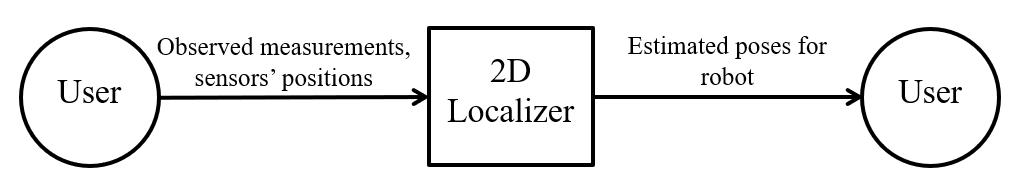
\includegraphics[width=0.6\textwidth]{SystemContextFigure.png}
\caption{System Context}
\label{Fig_SystemContext} 
\end{center}
\end{figure}
\begin{itemize}
\item User Responsibilities:
\begin{itemize}
\item Provide inputs including the coordinates of each environmental sensor and the measurements taken from them.
\item Evaluate the inputs to ensure all are their respective types
\end{itemize}
\item 2D Localizer Responsibilities:
\begin{itemize} 
\item Detect data type mismatch, such as a string of characters instead of a
  floating point number
\item Estimate the position and orientation of the robot
\end{itemize}
\end{itemize}

\subsection{User Characteristics}\label{SecUserCharacteristics}

The end user of 2D Localizer should have some familiarity with types of range sensors along with how to read and collect their data. They should also have basic experience with programming.

\subsection{System Constraints}

There are no system constraints.

\section{Specific System Description}

This section first presents the problem description, which gives a high-level
view of the problem to be solved.  This is followed by the solution characteristics
specification, which presents the assumptions, theories, definitions and finally
the instance models.

\subsection{Problem Description}\label{Sec_pd}

2D Localizer is intended to help keep track of mobile robots while carrying out their tasks.

\subsubsection{Terminology and  Definitions}

This subsection provides a list of terms that are used in the subsequent
sections and their meaning, with the purpose of reducing ambiguity and making it
easier to correctly understand the requirements:

\begin{itemize}

\item \textbf{Pose:} Position and orientation of the robot.
\item \textbf{Localization}: Determining where an object is with respect to its environment.
\item \textbf{Fiducial Markers (FMs)}: Markers placed around the environment for the robot to determine its location.
\item \textbf{Beacon}: A range sensor.

\end{itemize}

\subsubsection{Physical System Description}\label{sec_phySystDescrip}

The physical system of the localizer includes the following elements:

\begin{itemize}

\item[PS1:] The mobile robot

\item[PS2:] The beacons placed in the environment

\item[PS3:] The camera sensors on the mobile robot

\item[PS4:] The fiducial markers in the environment

\end{itemize}

\subsubsection{Goal Statements}

\noindent Given the imported 2D map, coordinates of all sensors and fiducial markers in the environment, and the noisy measurements of the sensors, the goal statements are:

\begin{itemize}

\item[GS\refstepcounter{goalnum}1\label{GS1}:] Calculate the estimated pose and error of the robot throughout its trajectory from sensors in the environment and on the robot.
\item[GS\refstepcounter{goalnum}2\label{GS2}:] Display a visual representation of the robot traversing the 2-D map with the sensors placed.

\end{itemize}

\subsection{Solution Characteristics Specification}

The instance models that govern 2D Localizer are presented in
Subsection~\ref{sec_instance}.  The information to understand the meaning of the
instance models and their derivation is also presented, so that the instance
models can be verified.

\subsubsection{Assumptions}\label{sec_assumpt}


This section simplifies the original problem and helps in developing the
theoretical model by filling in the missing information for the physical system.
The numbers given in the square brackets refer to the theoretical model [TM],
general definition [GD], data definition [DD], instance model [IM], or likely
change [LC], in which the respective assumption is used.

\begin{itemize}

\item[A\refstepcounter{assumpnum}1 \label{A_sensors}:]Robot uses camera sensors while the environment uses beacons and FMs (\tref{T_SE}, \ddref{DD_distance})
\item[A\refstepcounter{assumpnum}2 \label{A_controlled}:]Localizer is used in a controlled environment (i.e., indoors) (\tref{T_SE})
\item[A\refstepcounter{assumpnum}3 \label{A_indep}:]Each sensor has independent measurements, meaning the data from one does not depend on or affect the data from another. (\tref{T_FIM}, \iref{IM_like})
\item[A\refstepcounter{assumpnum}4 \label{A_noise}:]Sensor noise is zero-mean Gaussian (\tref{T_FIM}, \ddref{DD_distance})


\end{itemize}

\subsubsection{Theoretical Models}\label{sec_theoretical}

This section focuses on the general equations and laws that 2D Localizer is based
on.

~\newline
%TM 1
\noindent
\begin{minipage}{\textwidth}
\renewcommand*{\arraystretch}{1.5}
\begin{tabular}{| p{\colAwidth} | p{\colBwidth}|}
\hline
\rowcolor[gray]{0.9}
Number& TM\refstepcounter{theorynum}\thetheorynum\label{T_NRM}\\
\hline
Label &\bf Noisy Range Measurement \\
\hline
Equation& \begin{displaymath}
  g_j(x) = \lVert \mathbf{x_i} - \mathbf{a_j}\rVert + \eta_j
\end{displaymath} \\
\hline
Description &
The equation above gives the noisy range measurement $g_j$ (\si\metre) of the beacons placed in the environment (\aref{A_sensors}) where \\
& $\mathbf{x_i}$ is the position of the robot (\si\metre), \\
& $\mathbf{a_j}$ is the position of the beacon $j$ (\si\metre), and \\
& $\eta_j \sim \mathcal{N}(0, \sigma_j^2)$ is the noise from the $j$th beacon (\si\metre) (\aref{A_noise}).
\\
\hline
Source & \citet{Sequeira2024}\\
\hline
Ref.\ By & \ddref{DD_distance}\\
\hline
Preconditions & \aref{A_noise}\\
\hline
Derivation & None\\
\hline
\end{tabular}
\end{minipage}\\

% TM2
~\newline

\noindent
\begin{minipage}{\textwidth}
\renewcommand*{\arraystretch}{1.5}
\begin{tabular}{| p{\colAwidth} | p{\colBwidth}|}
\hline
\rowcolor[gray]{0.9}
Number& TM\refstepcounter{theorynum}\thetheorynum\label{T_FIM}\\
\hline
Label &\bf Fisher Information Matrix (FIM) \\
\hline
Equation& \begin{displaymath}
  \boldsymbol{\mathcal{I}} (\mathbf{\hat{x}}) \cong \sum_{j=1}^{N}\frac{1}{\sigma_j^2} \frac{\left(\mathbf{\hat{x}}-\mathbf{a_j}\right) \left( \mathbf{\hat{x}}-\mathbf{a_j}\right)^T}{\lVert \mathbf{\hat{x}}-\mathbf{a_j} \rVert^2}
\end{displaymath}\\
\hline
Description &
This equation gives the FIM which shows how much information the data provides about the robot's position \\
& $\sigma_j^2$ is the sensor variance used in the noise factor\\
& $\mathbf{a_j}$ is the position of beacon $j$ (\si\metre), and \\
& $\mathbf{\hat{x}}$ is the estimated position in \iref{IM_MLE} (\si\metre)\\
\hline
Source & \cite{Barfoot2017} \\
\hline
Ref.\ By & \tref{T_CRLB}\\
\hline
Preconditions & \aref{A_noise}, \iref{IM_MLE}\\
\hline
\end{tabular}
\end{minipage}\\

\subsubsection*{Derivation of FIM}

\tref{T_FIM} was derived from \dref{GD_PDF} and \iref{IM_like} as the FIM formula from \cite{Barfoot2017} is
\begin{displaymath}
  \boldsymbol{\mathcal{I}}(\mathbf{x} | \boldsymbol{\theta}) = \mathbb{E} \left[
\left( \frac{\partial \ln p(\mathbf{x} | \boldsymbol{\theta})}{\partial \boldsymbol{\theta}} \right)^{T}
\left( \frac{\partial \ln p(\mathbf{x} | \boldsymbol{\theta})}{\partial \boldsymbol{\theta}} \right)
\right]
\end{displaymath}

where\\ 
\[\frac{\partial \ln p(\mathbf{x} | \boldsymbol{\theta})}{\partial \boldsymbol{\theta}}\] is the score function which measures how much the likelihood changes from the parameter being estimated $\boldsymbol{\theta}$ from observed data $\mathbf{x}$.

To change it to the software's symbols, the FIM would be
\begin{displaymath}
  \boldsymbol{\mathcal{I}}(\mathbf{x}) = \mathbb{E} \left[
  \left( \frac{\partial \ln p(\mathbf{\tilde{d}} | \mathbf{x})}{\partial \mathbf{x}} \right)^{T}
  \left( \frac{\partial \ln p(\mathbf{\tilde{d}} | \mathbf{x})}{\partial \mathbf{x}} \right)
  \right]
\end{displaymath} 

Continuing with Barfoot's equations, their Gaussian Probability Density Function (PDF) can be made with \dref{GD_PDF} since it requires a mean and variance. This can be shown as
\begin{displaymath}
  p(\tilde{d_j} | \mathbf{x}) = \frac{1}{\sqrt{2\pi\sigma_j^2}} 
  \exp \left( 
  -\frac{(\tilde{d}_j - \lVert\mathbf{x} - \mathbf{a}_j\rVert)^2}{2\sigma_j^2} 
  \right)
\end{displaymath}

Linking it to \iref{IM_like}:
\begin{displaymath}
  p(\tilde{\mathbf{d}} | \mathbf{x}) = \prod_{j=1}^{N} 
  \frac{1}{\sqrt{2\pi\sigma_j^2}} 
  \exp \left( 
  -\frac{(\tilde{d}_j - \|\mathbf{x} - \mathbf{a}_j\|_2)^2}{2\sigma_j^2} 
  \right)
\end{displaymath}

From here, the log-likelihood function can be calculated:

\begin{displaymath}
  \ln p(\tilde{\mathbf{d}} | \mathbf{x}) = \sum_{j=1}^{N} 
  \left[ -\frac{1}{2} \ln (2\pi\sigma_j^2) 
  - \frac{(\tilde{d}_j - \|\mathbf{x} - \mathbf{a}_j\|_2)^2}{2\sigma_j^2} 
  \right]
\end{displaymath}

\begin{displaymath}
  \ln p(\tilde{\mathbf{d}} | \mathbf{x}) = -\sum_{j=1}^{N} 
  \frac{(\tilde{d}_j - \|\mathbf{x} - \mathbf{a}_j\|_2)^2}{2\sigma_j^2}
\end{displaymath}

The score function can then be written as

\begin{displaymath}
  \frac{\partial \ln p(\tilde{\mathbf{d}} | \mathbf{x})}{\partial \mathbf{x}} = \sum_{j=1}^{N} 
  \frac{(\tilde{d}_j - \|\mathbf{x} - \mathbf{a}_j\|_2)}{\sigma_j^2}
  \frac{\mathbf{x} - \mathbf{a}_j}{\|\mathbf{x} - \mathbf{a}_j\|}
\end{displaymath}

This function is in the expectation of FIM formula so when referring to \ddref{DD_distance} 

\begin{displaymath}
  \mathbb{E} \left[ \tilde{d}_j - \|\mathbf{x} - \mathbf{a}_j\|_2 \right] 
= \mathbb{E} \left[ \eta_j \right] = 0
\end{displaymath}

the noise has zero mean (\aref{A_noise}). Cancelling that portion out gives us this model, also known as \tref{T_FIM}

\begin{displaymath}
  \boldsymbol{\mathcal{I}}(\mathbf{x}) \cong \sum_{j=1}^{N}\frac{1}{\sigma_j^2} \frac{\left(\mathbf{x}-\mathbf{a_j}\right) \left( \mathbf{x}-\mathbf{a_j}\right)^T}{\lVert \mathbf{x}-\mathbf{a_j} \rVert^2}
\end{displaymath}

%TM3
~\newline

\noindent
\begin{minipage}{\textwidth}
\renewcommand*{\arraystretch}{1.5}
\begin{tabular}{| p{\colAwidth} | p{\colBwidth}|}
\hline
\rowcolor[gray]{0.9}
Number& TM\refstepcounter{theorynum}\thetheorynum\label{T_CRLB}\\
\hline
Label &\bf Cram\'{e}r-Rao Lower Bound (CRLB)\\
\hline
Equation& \begin{displaymath}
  Var( \mathbf{\hat{x}}) \geq \frac{1}{\boldsymbol{\mathcal{I}}(\mathbf{\hat{x}})}
\end{displaymath}\\
\hline
Description &
This equation gives the CRLB which shows how accurate an estimate of a parameter is given the noise in the measurements by providing a lower bound to the estimate's variance. We are able to use \tref{T_FIM} to get this lower bound \\
& $Var(\mathbf{\hat{x}})$ is the variance of the unbiased estimator in \iref{IM_MLE}\\
& $\boldsymbol{\mathcal{I}}(\mathbf{\hat{x}})$ is the FIM calculated from \tref{T_FIM}
\\
\hline
Source & \cite{Barfoot2017} \\
\hline
Ref.\ By & None\\
\hline
Preconditions & \tref{T_FIM}, \iref{IM_MLE}\\
\hline
Derivation & None\\
\hline
\end{tabular}
\end{minipage}\\

%TM4
~\newline

\noindent
\begin{minipage}{\textwidth}
\renewcommand*{\arraystretch}{1.5}
\begin{tabular}{| p{\colAwidth} | p{\colBwidth}|}
\hline
\rowcolor[gray]{0.9}
Number& TM\refstepcounter{theorynum}\thetheorynum\label{T_SE}\\
\hline
Label &\bf Special Euclidean (SE) 2 Transformation \\
\hline
Equation& \begin{displaymath}
  T_{robot} =  
    \begin{bmatrix}
      \mathbf{R}(\theta) & \mathbf{t} \\
      0 & 1\\
    \end{bmatrix}
    =
    \begin{bmatrix}
      \cos\theta & -\sin\theta & x\\
      \sin\theta & \cos\theta & y\\
      0 & 0 & 1\\
    \end{bmatrix}
\end{displaymath}\\
\hline
Description &
This equation shows SE(2) which represents all possible 2D transformations of the robot. Since the robot has cameras placed on it (\aref{A_sensors}), SE(2) can be used to get the position and orientation through the FMs. \\
& $\mathbf{R}(\theta)$ is the rotation represented as a 2$\times$2 matrix\\
& $\mathbf{t}$ is the translation represented as a 2$\times$1 matrix\\
& $[0~1]$ makes sure that the matrix is homogenous \\
& $x,y$ are the positions for the $x$ and $y$ coordinates of the 2D map
\\
\hline
Source & \cite{Barfoot2017} \\
\hline
Ref.\ By & None\\
\hline
Preconditions & None\\
\hline
Derivation & None\\
\hline
\end{tabular}
\end{minipage}\\

~\newline

\subsubsection{General Definitions}\label{sec_gendef}
This section collects the laws and equations that will be used in building the
instance models.

~\newline

\noindent
\begin{minipage}{\textwidth}
\renewcommand*{\arraystretch}{1.5}
\begin{tabular}{| p{\colAwidth} | p{\colBwidth}|}
\hline
\rowcolor[gray]{0.9}
Number& GD\refstepcounter{defnum}\thedefnum\label{GD_PDF}\\
\hline
Label &\bf Probability Density Function (PDF)\\
\hline
% Units&$MLt^{-3}T^0$\\
% \hline
SI Units&\si{\per\metre}\\
\hline
Equation&\begin{displaymath}
  p_j \left( \tilde{d_j}\vert \mathbf{x} \right) = \mathcal{N}\left( \lVert \mathbf{x} - \mathbf{a_j} \rVert, \sigma_j^2 \right)
\end{displaymath}  \\
\hline
Description & This definition is about the Gaussian PDF (\aref{A_noise}) being used in \iref{IM_like}. This provides the PDF of the actual noisy range measurement $\tilde{d_j}$ of beacon $j$ (\ddref{DD_distance}) that is conditioned on the robot's position $\mathbf{x}$.\\
& $\mathcal{N}$ is the normal distribution with $\lVert \mathbf{x} - \mathbf{a_j} \rVert$ as the mean (predicted range) and $\sigma_j^2$ as the variance.
\\
\hline
  Source &\cite{Sequeira2024} \\
  \hline
  Ref.\ By & \iref{IM_like}\\
  \hline
\end{tabular}
\end{minipage}\\

\subsubsection{Data Definitions}\label{sec_datadef}

This section collects and defines all the data needed to build the instance
models. The dimension of each quantity is also given.
~\newline

\noindent
\begin{minipage}{\textwidth}
\renewcommand*{\arraystretch}{1.5}
\begin{tabular}{| p{\colAwidth} | p{\colBwidth}|}
\hline
\rowcolor[gray]{0.9}
Number& DD\refstepcounter{datadefnum}\thedatadefnum\label{DD_distance}\\
\hline
Label& \bf Actual Range Measurement\\
\hline
Symbol &$\tilde{d_j}$\\
% Units& $Mt^{-3}$\\
\hline
  SI Units & \si{\metre}\\
  \hline
  Equation& \begin{displaymath}
    \tilde{d_j} = \lVert \mathbf{x_i} - \mathbf{a_j}\rVert + \eta_j
  \end{displaymath}\\
  \hline
  Description & 
  $\tilde{d_j}$ is the actual beacon measurement that will be used compared to \tref{T_NRM} which is just a model. Although it would return a scalar from the sensor, the formulation the equation above. \\
  & $\mathbf{x_i}$ is the position of the robot (\si\metre), \\
  & $\mathbf{a_j}$ is the position of the $j$th beacon placed (\si\metre), and \\
  & $\eta_j \sim \mathcal{N}(0, \sigma_j^2)$ is the noise from beacon $j$ (\si\metre) (\aref{A_noise}).
  \\
  \hline
  Sources&\cite{Sequeira2024} \\
  \hline
  Ref.\ By &\dref{GD_PDF}\\
  \hline
\end{tabular}
\end{minipage}\\

% ~\newline

% \noindent
% \begin{minipage}{\textwidth}
% \renewcommand*{\arraystretch}{1.5}
% \begin{tabular}{| p{\colAwidth} | p{\colBwidth}|}
%   \hline
%   \rowcolor[gray]{0.9}
%   Type Name & Name for Type\\
%   \hline
%   Type Def & mathematical definition of the type\\
%   \hline
%   Description & description here
%   \\
%   \hline
%   Sources & Citation here, if the type is borrowed from another source\\
%   \hline
% \end{tabular}
% \end{minipage}\\

\subsubsection{Instance Models}\label{sec_instance}    
This section transforms the problem defined in Section~\ref{Sec_pd} into 
one which is expressed in mathematical terms. It uses concrete symbols defined 
in Section~\ref{sec_datadef} to replace the abstract symbols in the models 
identified in Sections~\ref{sec_theoretical} and~\ref{sec_gendef}.

The goal \gsref{GS1} is solved by \iref{IM_like} and \iref{IM_MLE}.

~\newline

%Instance Model 1

\noindent
\begin{minipage}{\textwidth}
\renewcommand*{\arraystretch}{1.5}
\begin{tabular}{| p{\colAwidth} | p{\colBwidth}|}
  \hline
  \rowcolor[gray]{0.9}
  Number& IM\refstepcounter{instnum}\theinstnum\label{IM_like}\\
  \hline
  Label& \bf Joint Likelihood Function \\
  \hline
  Input&$\mathbf{\tilde{d}}$, $N$\\
  \hline
  Output& $p ( \mathbf{\tilde{d}} \vert \mathbf{x} ) $\\
  \hline
  Equation&\begin{displaymath}
    p \left( \mathbf{\tilde{d}} \vert \mathbf{x} \right) = \prod_{j=1}^{N} p\left( \tilde{d_j}\vert \mathbf{x} \right)
  \end{displaymath}\\
  \hline
  Description& This equation uses the measurements gotten from each beacon (\aref{A_indep}) to calculate the product of how likely $\mathbf{x}$ is the best position to reflect the inputs where \\
  & $\mathbf{\tilde{d}} = [ \tilde{d_1}, \tilde{d_2}, \dots, \tilde{d_N}]$, \\
  & N is the number of beacons, and \\
  & $p( \tilde{d_j}\vert \mathbf{x})$ is the Gaussian PDF from \dref{GD_PDF}
  \\
  \hline
  Sources& \cite{Sequeira2024} \\
  \hline
  Ref.\ By & \iref{IM_MLE}\\
  \hline
\end{tabular}
\end{minipage}\\

~\newline

%IM 2
\noindent
\begin{minipage}{\textwidth}
\renewcommand*{\arraystretch}{1.5}
\begin{tabular}{| p{\colAwidth} | p{\colBwidth}|}
  \hline
  \rowcolor[gray]{0.9}
  Number& IM\refstepcounter{instnum}\theinstnum\label{IM_MLE}\\
  \hline
  Label& \bf Maximum Likelihood Estimation (MLE) \\
  \hline
  Input&$p( \mathbf{\tilde{d}} \vert \mathbf{x} )$\\
  \hline
  Output& $\mathbf{\hat{x}} $\\
  \hline
  Equation&\begin{displaymath}
    \mathbf{\hat{x}} = \underset{x}{\arg\max}\,p( \mathbf{\tilde{d}} \vert \mathbf{x} )
  \end{displaymath}\\
  \hline
  Description&Continuing from \iref{IM_like}, the MLE equation gives an estimate based on the maximum probability calculated from the joint likelihood function.\\
  & $ p( \mathbf{\tilde{d}} \vert \mathbf{x} )$ is the joint likelihood function from \iref{IM_like}\\
  \hline
  Sources& \cite{Sequeira2024} \\
  \hline
  Ref.\ By & \tref{T_FIM}, \tref{T_CRLB}\\
  \hline
\end{tabular}
\end{minipage}\\

~\newline


\subsubsection{Input Data Constraints} \label{sec_DataConstraints}    

Table~\ref{TblInputVar} shows the data constraints on the input output
variables.  The column for physical constraints gives the physical limitations
on the range of values that can be taken by the variable.  The column for
software constraints restricts the range of inputs to reasonable values.  The
software constraints will be helpful in the design stage for picking suitable
algorithms.  The constraints are conservative, to give the user of the model the
flexibility to experiment with unusual situations.  The column of typical values
is intended to provide a feel for a common scenario.  The uncertainty column
provides an estimate of the confidence with which the physical quantities can be
measured.  This information would be part of the input if one were performing an
uncertainty quantification exercise.

% The specification parameters in Table~\ref{TblInputVar} are listed in
% Table~\ref{TblSpecParams}.

\begin{table}[!h]
  \caption{Input Variables} \label{TblInputVar}
  \renewcommand{\arraystretch}{1.2}
\noindent \begin{longtable*}{l l l l c} 
  \toprule
  \textbf{Var} & \textbf{Physical Constraints} & \textbf{Software Constraints} &\textbf{Typical Value} & \textbf{Uncertainty}\\
  \midrule 
  $\mathbf{a_j}$ & $ \mathbf{a_j}> [0~0]$ & - & [1.5, 2.6] \si[per-mode=symbol] {\metre} & -
  \\
  $\tilde{d_j}$ & $ \tilde{d_j} > 0$ & - & 4.76 \si[per-mode=symbol] {\metre} & $\eta_j$
  \\
  \bottomrule
  \multicolumn{5}{l}{\scriptsize * The user will set up a series to insert rows of inputs.}\\
\end{longtable*}
\end{table}

% \noindent 
% \begin{description}
% \item[(*)] \plt{you might need to add some notes or clarifications}
% \end{description}

% \begin{table}[!h]
% \caption{Specification Parameter Values} \label{TblSpecParams}
% \renewcommand{\arraystretch}{1.2}
% \noindent \begin{longtable*}{l l} 
%   \toprule
%   \textbf{Var} & \textbf{Value} \\
%   \midrule 
%   $L_\text{min}$ & 0.1 \si{\metre}\\
%   \bottomrule
% \end{longtable*}
% \end{table}

\subsubsection{Properties of a Correct Solution}\label{sec_CorrectSolution}

\noindent
A correct solution must exhibit

\begin{table}[!h]
\caption{Output Variables}\label{TblOutputVar}
\renewcommand{\arraystretch}{1.2}
\noindent \begin{longtable*}{l l} 
  \toprule
  \textbf{Var} & \textbf{Physical Constraints} \\
  \midrule 
  $\mathbf{\hat{x}}$ & $\mathbf{\hat{x}} > [0~0]$
  \\
  \bottomrule
\end{longtable*}
\end{table}

\section{Requirements}

This section provides the functional requirements, the business tasks that the
software is expected to complete, and the nonfunctional requirements, the
qualities that the software is expected to exhibit.

\subsection{Functional Requirements}

\noindent\begin{itemize}

\item[R\refstepcounter{reqnum}\thereqnum\label{R_Inputs}:] Provide the inputs for 2D Localizer which include the 2D map, the coordinates of all sensors and markers located in the environment, and the measurements taken from the sensors.

\item[R\refstepcounter{reqnum}\thereqnum\label{R_OutputInputs}:] 2D Localizer will acquire $\mathbf{\hat{x}}$ from the inputs in \rref{R_Inputs}.

\item[R\refstepcounter{reqnum}\thereqnum\label{R_Calculate}:] 2D Localizer will calculate the estimated posed from the measurements provided for \iref{IM_MLE}.

\item[R\refstepcounter{reqnum}\thereqnum\label{R_VerifyOutput}:] 2D Localizer will verify that inputs provided are within their constraints.

\item[R\refstepcounter{reqnum}\thereqnum\label{R_Output}:] 2D Localizer will show a visual animated graph that tracks the mobile robots work while also displaying the sensors' coordinates.

\end{itemize}

\subsection{Nonfunctional Requirements}

This problem priorities the accuracy of the estimations along with its performance when it comes to keeping up with the robot's movements. That being said, the nonfunctional requirements are:

\noindent \begin{itemize}

\item[NFR\refstepcounter{nfrnum}\thenfrnum \label{NFR_Accuracy}:]
  \textbf{Accuracy}: The accuracy of the computed estimations should meet the threshold when comparing to the predicted measurements. 

\item[NFR\refstepcounter{nfrnum}\thenfrnum \label{NFR_Understandibility}:] \textbf{Understandability}: The software should be simple to understand and implement.

\item[NFR\refstepcounter{nfrnum}\thenfrnum \label{NFR_Maintainability}:]
  \textbf{Maintainability}: The software should be simple modify some components when needed.

\item[NFR\refstepcounter{nfrnum}\thenfrnum \label{NFR_Reusability}:]
  \textbf{Usability}: The software should be easy to run and have minimal troubleshooting.
\end{itemize}

\subsection{Rationale}

This program has rationale for the assumptions mentioned in~\ref{sec_assumpt}:
\begin{itemize}
  \item \aref{A_sensors}: Assuming the type of sensors assisted in setting up the type of output variables that is needed for each set of estimates.
  \item \aref{A_controlled}: Referring to \aref{A_sensors}, vision sensors will be used on the robot and lighting could affect the way they detect FMs. Another main reason for this assumption is so that the coordinates of each beacon and FM can be structured around the area the user provides.
  \item \aref{A_indep}: To find the sum and products of variables that need data from each beacon and FM placement (\tref{T_FIM}, \iref{IM_like}), having each sensor collect independent data from different positions would help with the overall accuracy the program would want to achieve.
  \item \aref{A_noise}: The most common way to model noise in robotics is with a Gaussian distribution, making it a reasonable and sufficient assumption for this software.
\end{itemize}

\section{Likely Changes}    

There are no likely changes to be made.

% \noindent \begin{itemize}

% \item[LC\refstepcounter{lcnum}\thelcnum\label{LC_meaningfulLabel1}:] \plt{Give
%     the likely changes, with a reference to the related assumption (aref), as appropriate.}

% \end{itemize}

\section{Unlikely Changes}    

\noindent \begin{itemize}

\item[UC\refstepcounter{ucnum}\theucnum\label{UC_noise}:] \aref{A_noise} There are various models that are derived based on the Gaussian noise meaning that it would be detrimental to change.

\end{itemize}

\section{Traceability Matrices and Graphs}

The purpose of the traceability matrices is to provide easy references on what
has to be additionally modified if a certain component is changed.  Every time a
component is changed, the items in the column of that component that are marked
with an ``X'' may have to be modified as well.  Table~\ref{Table:trace} shows the
dependencies of theoretical models, general definitions, data definitions, and
instance models with each other. Table~\ref{Table:R_trace} shows the
dependencies of instance models, requirements, and data constraints on each
other. Table~\ref{Table:A_trace} shows the dependencies of theoretical models,
general definitions, data definitions, instance models, and likely changes on
the assumptions.

% \begin{landscape}

% \end{landscape}

\begin{table}[h!]
\centering
\begin{tabular}{|c|c|c|c|c|c|c|c|c|c|c|}
\hline        
	& \tref{T_NRM}& \tref{T_FIM}& \tref{T_CRLB}& \tref{T_SE} & \dref{GD_PDF}& \ddref{DD_distance} & \iref{IM_like} & \iref{IM_MLE}\\
\hline
\tref{T_NRM}         & & & & & & & & \\ \hline
\tref{T_FIM}         & & & & & X& &X &X \\ \hline
\tref{T_CRLB}        & & X& & & & & & X\\ \hline
\tref{T_SE}          & & & & & & & &  \\ \hline
\dref{GD_PDF}        & & & & & & & & \\ \hline
\ddref{DD_distance}  & X& & & & & & & \\ \hline
\iref{IM_like}       & & & & &X &X & & \\ \hline
\iref{IM_MLE}        & & & & & & &X &\\
\hline
\end{tabular}
\caption{Traceability Matrix Showing the Connections Between Items of Different Sections}
\label{Table:trace}
\end{table}

\begin{table}[h!]
\centering
\begin{tabular}{|c|c|c|c|c|c|c|c|}
\hline
	& \iref{IM_like}& \iref{IM_MLE}& \rref{R_Inputs}& \rref{R_OutputInputs}& \rref{R_Calculate}& \rref{R_VerifyOutput}& \rref{R_Output} \\
\hline
\iref{IM_like}          & & & & & & & \\ \hline
\iref{IM_MLE}           & X& & & & & & \\ \hline
\rref{R_Inputs}         & & & & & & & \\ \hline
\rref{R_OutputInputs}   & & & X& & & & \\ \hline
\rref{R_Calculate}      & & X& & & & & \\ \hline
\rref{R_VerifyOutput}   & & & & & & & \\ \hline
\rref{R_Output}         & & & & & & & \\
\hline
\end{tabular}
\caption{Traceability Matrix Showing the Connections Between Requirements and Instance Models}
\label{Table:R_trace}
\end{table}

\begin{table}[h!]
\centering
\begin{tabular}{|c|c|c|c|c|}
\hline
	& \aref{A_sensors}& \aref{A_controlled}& \aref{A_indep}& \aref{A_noise} \\
\hline
\tref{T_NRM}         &X & & &X  \\ \hline
\tref{T_FIM}         & & &X &X  \\ \hline
\tref{T_CRLB}        & & & &  \\ \hline
\tref{T_SE}          &X &X & &  \\ \hline
\dref{GD_PDF}        & & & & X \\ \hline
\ddref{DD_distance}  & & & &X \\ \hline
\iref{IM_like}       & & &X & \\ \hline
\iref{IM_MLE}        & & & & \\ \hline
\ucref{UC_noise}     & & & &X\\
\hline
\end{tabular}
\caption{Traceability Matrix Showing the Connections Between Assumptions and Other Items}
\label{Table:A_trace}
\end{table}

\clearpage

\bibliographystyle{plainnat}
\bibliography{mybib}

\end{document}